\documentclass[aps,prapplied,reprint,superscriptaddress]{revtex4-2}
\raggedbottom

\usepackage{amsmath,amssymb}
\usepackage{graphicx}
\usepackage{booktabs}
\usepackage{tabularx}
\usepackage{array}
\usepackage{enumitem}
\usepackage{xcolor}
\usepackage{url}
\usepackage{tikz}
\usetikzlibrary{shapes.geometric, arrows.meta, positioning, fit, backgrounds}

\graphicspath{{figures/}{../cross_sim/figures/}}

\newcommand{\DG}{\Delta G}
\newcommand{\Areq}{A_{\rm req}}
\newcommand{\Aqual}{A_{\rm qual}}
\newcommand{\HB}{H_{\rm B}}

\begin{document}

\title{Assessing Decision Reliability in Discrete-Event Simulation:\\A Quantum-Network Case Study}

\author{David Vesterlund}
\affiliation{Vesterlund Ventures, WestQuant Open}
\email{david@vesterlundventures.se}

\date{8 October 2026}

\thanks{ORCID: 0009-0000-6455-1141}

\begin{abstract}
Simulation-based design decisions depend on stochastic variation, analyst choices, and model semantics. We present a workflow that separates these sources of uncertainty using a canonical experiment specification, independent seed pools, explicit intervention gains, and distinct measures of numerical, ranking, decision, and claim agreement. A quantum-network case study compares an author-developed simulator with a harmonized reference model; two framework adapters share the same reference logic and do not constitute independent model replications. Across 400 configurations, a reported two-pool experiment increases label agreement from 71.5\% with a single seed to 95.8\% with 20-seed averaging. The full protocol and simple averaging achieve the same agreement, so the improvement is attributable to replication rather than a uniquely superior labeling rule. Separate analyses show sensitivity to intervention strength and performance definitions. In a finite-grid memory analysis, 50.8\% of 356 matched interior cases differ by at least a factor of four between model variants, with a configuration-clustered 95\% interval of 37.4--63.9\%. This empirical comparison is conditional on its metric, retained configurations, and shared implementation assumptions. The methodological contribution is an auditable separation of within-model repeatability, between-model sensitivity, and metric incompatibility. We provide reporting requirements and a staged verification plan; full native-protocol and hardware validation remain future work.
\end{abstract}

\maketitle

% ============================================================
\section{Introduction}
\label{sec:intro}

Quantum-network design requires deciding which physical resource to improve first: memory capacity, generation rate, retrieval efficiency, coherence time, or routing. A natural approach is \emph{intervention-based bottleneck identification}: improve each resource by a fixed amount, measure the marginal performance gain $\DG_j$, and label the bottleneck as the resource with the largest $\DG_j$. This approach is intuitive, model-agnostic, and produces a single actionable label.

But how robust is that label? A reviewer of any such analysis should ask: would the label change with a different random seed? With a larger or smaller intervention? With a different performance metric or fidelity threshold? With a different simulator?

A growing number of discrete-event simulators---NetSquid~\cite{coopmans2021netsquid}, SeQUeNCe~\cite{wu2021sequence}, QuISP~\cite{satoh2022quisp}, SimQN~\cite{chen2023simqn}---offer different modeling choices for the same physical phenomena. When different models are applied to the same problem, they may produce different numerical predictions. This is not a bug; it is a consequence of the fact that simulation is an abstraction. The question is not whether simulators disagree---they inevitably do---but \emph{which types of scientific conclusions survive a change of simulation model, and which do not}.

\subsection{Simulator Output as a Function of Assumptions, Semantics, and Implementation}

A simulator's output depends on three layers:

\begin{enumerate}[leftmargin=2em]
\item \textbf{Model assumptions:} The physical and mathematical models (noise model, generation model, swapping model). These are typically well-documented in publications.
\item \textbf{Protocol semantics:} The operational definitions of what constitutes a ``completed request,'' when a latency clock starts, how waiting and queueing work, when memory slots are locked and released, whether generation is sequential or concurrent, and how deadlines and censoring are handled. These are often \emph{implicit} and may differ between simulators without being documented.
\item \textbf{Implementation:} The software engineering (event scheduling, RNG, numerical precision, data structures). These affect reproducibility but not (in principle) scientific conclusions.
\end{enumerate}

This distinction is critical. Two simulators that share the same model assumptions but differ in protocol semantics may produce different scientific conclusions. Two simulators that share both model assumptions and protocol semantics but differ in implementation should produce identical results (up to numerical precision). We therefore write simulator output as:
\begin{equation}
\begin{aligned}
y ={}& f(x,\; \text{model assumptions},\\
      & \text{protocol semantics},\; \text{implementation}).
\end{aligned}
\end{equation}
and the trustworthiness of any conclusion depends on which of these factors it is sensitive to. This reframes the question from ``which simulator is best?'' to ``what should a trustworthy quantum-network simulator guarantee for this conclusion to be reliable?''

\subsection{Four Types of Agreement}
\label{sec:four_agreement}

A central conceptual contribution is the distinction between four types of cross-simulator agreement, which are often conflated (Figure~\ref{fig:agreement}):

\begin{figure}[t]
\centering
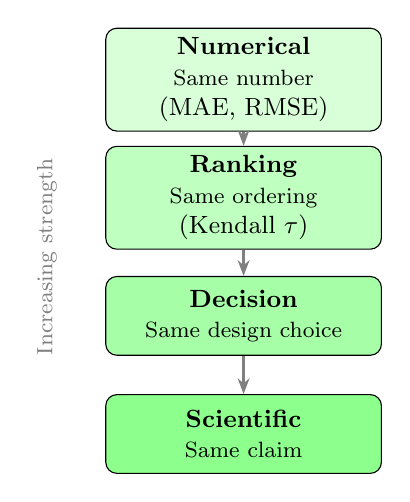
\begin{tikzpicture}[
  box/.style={draw, rounded corners, minimum width=3.5cm, minimum height=1cm, font=\small, align=center},
  arrow/.style={-{Stealth[length=2mm]}, thick, gray}
]
\node[box, fill=green!15] (num) at (0, 3) {\textbf{Numerical}\\\footnotesize Same number\\(MAE, RMSE)};
\node[box, fill=green!25] (rank) at (0, 1.5) {\textbf{Ranking}\\\footnotesize Same ordering\\(Kendall $\tau$)};
\node[box, fill=green!35] (dec) at (0, 0) {\textbf{Decision}\\\footnotesize Same design choice};
\node[box, fill=green!45] (sci) at (0, -1.5) {\textbf{Scientific}\\\footnotesize Same claim};
\draw[arrow] (num) -- (rank);
\draw[arrow] (rank) -- (dec);
\draw[arrow] (dec) -- (sci);
\node[font=\footnotesize, gray, rotate=90] at (-2.5, 0.75) {Increasing strength};
\end{tikzpicture}
\caption{Four types of cross-simulator agreement, ordered by strength. Numerical agreement is the weakest; scientific-conclusion agreement is the strongest. Two simulators can have high numerical agreement but low decision agreement (small differences near a threshold flip the decision). Each main result in this paper is reported on all four levels.}
\label{fig:agreement}
\end{figure}

\begin{enumerate}[leftmargin=2em]
\item \textbf{Numerical agreement:} Two simulators produce the same number (or nearly the same number) for a given metric. Measured by MAE, RMSE, or relative error.
\item \textbf{Ranking agreement:} Two simulators produce the same ordering of configurations. Measured by Kendall $\tau$ or Spearman $\rho$.
\item \textbf{Decision agreement:} Two simulators lead to the same design decision (e.g., the same memory family is selected, the same topology is preferred). Measured by decision-changing disagreement rates.
\item \textbf{Scientific-conclusion agreement:} Two simulators support the same scientific claim (e.g., ``memory family A outperforms B,'' ``throughput increases monotonically with memory,'' ``scalar collapse fails''). This is the strongest form of agreement and the one that matters for science.
\end{enumerate}

These four types are not interchangeable. Two simulators can have low numerical agreement but high ranking agreement (all values are shifted by a constant factor, but the ordering is preserved). Two simulators can have high numerical agreement but low decision agreement (small differences near a threshold flip the decision). Throughout this paper, each main result is reported on all four levels where applicable.

\subsection{Contributions}

\begin{enumerate}[leftmargin=2em]
\item A unified fragility framework measuring three axes---noise, analyst choices, and model switching---on a shared Canonical Experiment Specification, with each result reported on four agreement levels.
\item A benchmark ladder (B0--B6) with the rule that each step must be passed before the next runs, replacing the ad-hoc CV0--CV7 ladder.
\item A semantic-dimensions table covering only the two systems actually run (WestQuant and SeQUeNCe), identifying which semantic choices are switchable and which are definition mismatches.
\item Empirical evidence that the dominant bottleneck label is fragile: 50.7\% of configurations show at least one seed disagreement at 2000 requests; 63\% of short-run changes are statistically tied.
\item A factorial design over semantic switches showing that retrieval-in-delivery explains 72\% of $A_{\rm req}$ variance for AFC, but this measures $A_{\rm req}$ variance across configurations (including $m$ and $\lambda$), not model disagreement. With all seven interventions, $\kappa = 0.055$ (retrieval on) and $\kappa = 0.000$ (retrieval matched); retrieval matching does not improve agreement.
\item A three-class taxonomy of conclusion reproducibility: structural (reproduced), model-sensitive (not reproduced), and definition-sensitive (non-comparable).
\item A decision-transfer experiment showing 0\% transfer with retrieval on and 15\% with retrieval matched; $m_c$ disagreement (ratio $\geq 4\times$) is 85\% in both conditions.
\item A Trust Stack checklist for reporting, with reviewer recommendations.
\end{enumerate}

% ============================================================
\section{Setup: Common Experiment Specification and Validation Ladder}
\label{sec:setup}

\subsection{Canonical Experiment Specification}

When two simulators are given ``the same'' scenario, they may still produce different results because the scenario was translated differently. Different RNG implementations generate different arrival traces. Different topology representations assign different node labels. This creates \emph{false disagreement}---apparent simulator differences that are actually translation artifacts.

A Canonical Experiment Specification (CES) eliminates false disagreement by specifying every parameter before translation to any implementation. The CES defines:

\begin{itemize}[leftmargin=2em]
\item \textbf{Network:} Topology graph, node count, link distances.
\item \textbf{Hardware:} Memory family, $T_1$, $T_2$, retrieval efficiency, readout fidelity.
\item \textbf{Memory:} Capacity $m$, slot model, aging model.
\item \textbf{Links:} Generation probability $p_{\rm gen}$, attempt time, loss model.
\item \textbf{Traffic:} Arrival process, arrival rate $\lambda$, source-destination pairs, deadline.
\item \textbf{Protocol:} Swapping probability, purification, scheduling.
\item \textbf{Routing:} Path selection algorithm.
\item \textbf{Noise:} Depolarization, amplitude damping, readout errors.
\item \textbf{Metrics:} Definitions of throughput, fidelity, latency, resource use.
\item \textbf{Randomness:} Seeds, RNG algorithm, exogenous generation outside simulators.
\end{itemize}

The CES is simulator-neutral: it does not use any simulator's parameter names or data structures. Each simulator provides a translator that maps CES parameters to its own configuration format. Exogenous randomness (topology, arrivals, source-destination pairs) is generated outside the simulators to eliminate false disagreement from different RNG implementations. Each scenario uses three independent seed streams: (i) a \emph{graph seed} for topology generation, (ii) a \emph{traffic seed} for request arrivals and source-destination pairs, and (iii) a \textbf{physics seed} for link generation outcomes, swap outcomes, and decoherence realizations.

\subsection{Validation Ladder B0--B6}
\label{sec:ladder}

We propose a benchmark ladder for quantum-network simulation, with the rule that \emph{each step must be passed before the next runs}. Table~\ref{tab:benchmarks} summarizes the ladder and the validation criterion for each level.

\begin{table*}[t]
\centering
\caption{Benchmark ladder B0--B6. Each step must be passed before the next runs. B6 in this study is claim-level replication; hardware-calibrated validation (hardware-calibrated validation) remains future work.}
\label{tab:benchmarks}
\begin{tabular}{clp{4.5cm}p{4.5cm}r}
\toprule
Level & Name & Description & Validation Criterion & Scenarios \\
\midrule
B0 & Analytical primitives & Single-link generation, loss, decoherence & Match analytical rate formulas ($\epsilon_{\rm abs} < 0.05$) & 90 \\
B1 & Elementary entanglement & Two-node entanglement generation, memory families & Match analytical or experimental rates & 180 \\
B2 & Three-node repeater & Single swap, finite memory & Match analytical swapping formulas & 360 \\
B3 & Multi-hop chain & $N$-hop chain, path length scaling & Monotonicity, rate decay & 180 \\
B4 & Finite memory + contention & Memory limit, queueing, multiple requests & Cross-simulator ranking agreement ($\tau$) & 200 \\
B5 & Heterogeneous topology + traffic & Multiple topologies, stochastic traffic & Structural conclusion agreement & 60 \\
B6 & Claim-level replication & Full claim grid (C1--C5) across model families & Conclusion-level reproducibility & 2{,}880 \\
\bottomrule
\end{tabular}
\end{table*}

The ladder is cumulative: a simulator that passes B4 has also passed B0--B3. The hardest level (B6) requires claim-level replication across model families. Hardware-calibrated validation against experimental data is a further level that remains future work; we do not have experimental data for contention-dominated scenarios.

\textbf{B0 analytical verification gate.} B0 tests single-link generation with parameterized $p_{\rm gen}$, $T_2$, and retrieval efficiency $\eta$. For a single link without contention and without retrieval loss, the analytical completion rate is $\Areq = 1.0$. The harmonized model passes this gate because it treats retrieval as free ($\eta_r = 1$). WestQuant shows lower $\Areq$ (mean $0.65$) because it counts retrieval efficiency $\eta_r$ in the delivery: a request is dropped if retrieval fails ($\eta_r < 1$). The analytical reference of $1.0$ is correct only for a model that omits retrieval loss; a model that includes retrieval loss should give $\Areq = \eta_r$, not $1.0$. The B0 gate therefore rewards the model that omits the loss. This is a model-semantic effect (the \texttt{retrieval\_in\_delivery} switch, Sec.~\ref{sec:switches_1000}), not a physics error. WestQuant is retained because its retrieval semantics represent a deliberate modeling choice.

\subsection{Simulator Frameworks}

\textbf{WestQuant} is the native simulator. It models quantum networks with per-node memory capacity $m$, Bernoulli link generation, depolarizing noise, entanglement swapping, and concurrent request processing with queueing. When all memory slots at a node are occupied, incoming requests queue until a slot frees, incurring queueing delays that affect latency and memory aging.

\textbf{SeQUeNCe and SimQN (Harmonized Mode)} are used via harmonized adapters: their event engines are instantiated, but the physics logic is implemented in a shared harmonization layer using the same Bernoulli generation, depolarizing noise, and sequential blocking model. When memory is full, requests are rejected immediately rather than queued.

\textbf{Event-trace audit.} The SeQUeNCe and SimQN adapters produce bit-identical event traces across all tested scenarios (verified by SHA-256 hashing). The comparison is therefore effectively between one native model (WestQuant: concurrent generation + queueing) and one harmonized reference model (serial generation + immediate blocking), with $S_{\rm models} = 2$ rather than 3. Treating SeQUeNCe and SimQN as two independent models would constitute pseudoreplication.

\textbf{Native SeQUeNCe pilot.} A native SeQUeNCe adapter was developed as a pilot, instantiating SeQUeNCe's own \texttt{RouterNetTopo}, \texttt{QuantumRouter}, \texttt{BSMNode}, and \texttt{RequestApp} components. This adapter uses SeQUeNCe's own components but does not execute native protocol events; it is therefore a partial validation, not a full native comparison. The pilot ran 3 scenarios $\times$ 3 seeds = 9 scenario-seed pairs. Native SeQUeNCe produces different $\Areq$ values from WestQuant in several cases (e.g., chain $N{=}3$ $m{=}2$: WQ 0.889 vs.\ native 0.667), confirming that the adapter produces different values from WestQuant. However, the pilot is too small for statistical comparison (wall time $\sim$24--86\,s per scenario vs.\ $<$0.01\,s for WestQuant). A larger independent-judge experiment (25 configurations $\times$ 10 seeds = 250 runs) is reported in Section~\ref{sec:judge}; it also uses SeQUeNCe components but does not execute native protocol events, so it remains a partial validation.

\subsection{Performance Metrics}

All implementations report three primary metrics, computed over the observation window $[t_{\rm warmup}, T_{\rm obs}]$ with warmup excluded:

\begin{align}
\Areq &= \frac{N_{\rm completed}}{N_{\rm arrived}} \\
\Aqual &= \frac{N_{\rm completed} \cap N_{\rm qualified}}{N_{\rm arrived}} \\
R_{\rm qual} &= \frac{N_{\rm completed} \cap N_{\rm qualified}}{T_{\rm obs} - t_{\rm warmup}}
\end{align}

where $N_{\rm arrived}$ is the number of requests that entered the system during the observation window, $N_{\rm completed}$ are requests that reached the destination within the deadline $D = 10$\,s, and $N_{\rm qualified}$ are completed requests whose end-to-end fidelity $F \geq F_{\rm min} = 0.5$. $T_{\rm obs} = 200$\,s is the observation horizon and $t_{\rm warmup} = 20$\,s is excluded. $\Areq$ and $\Aqual$ are fractions in $[0, 1]$; $R_{\rm qual}$ is a rate.

\subsection{Intervention-Based Bottleneck Identification}

Given a network configuration $\theta$ and a performance metric $G(\theta)$, we define the \emph{intervention gain} for resource $j$ as
\begin{equation}
\DG_j(\theta, \delta) = G(T_{j,\delta}(\theta)) - G(\theta),
\end{equation}
where $T_{j,\delta}$ is an explicit intervention operator that improves resource $j$ by a relative amount $\delta$. The \emph{soft bottleneck vector} is
\begin{equation}
p_j = \frac{\max(0, \DG_j)}{\sum_k \max(0, \DG_k)},
\end{equation}
and the \emph{dominant bottleneck} is $\arg\max_j p_j$. The bottleneck entropy $\HB = -\sum_j p_j \log p_j$ measures how diffuse the bottleneck is. If all $\DG_j \leq \varepsilon$ ($\varepsilon = 10^{-6}$), the configuration is labeled \emph{degenerate}.

We study seven resources: \textbf{capacity} (memory slots), \textbf{generation} (success probability), \textbf{retrieval} (readout efficiency), \textbf{coherence} (decoherence rate), \textbf{routing} (policy), \textbf{deadline} (time limit), and \textbf{topology} (edge density).

\subsection{Agreement Measures}

We use four agreement measures, corresponding to the four types in Section~\ref{sec:four_agreement}:
\begin{itemize}[leftmargin=2em]
\item \textbf{Numerical:} MAE or RMSE against reference.
\item \textbf{Ranking:} Kendall $\tau$ for rankings of the soft vector.
\item \textbf{Decision:} Cohen's $\kappa$ for dominant labels; decision-changing disagreement rates.
\item \textbf{Scientific conclusion:} classification as structural, model-sensitive, or definition-sensitive.
\end{itemize}
We also report Jensen--Shannon distance for the full soft vector distributions.

% ============================================================
\section{Noise: Stochastic Fragility}
\label{sec:noise}

\subsection{Stratified Sample}

We generate a stratified sample of 400 configurations covering 6 memory families (trapped ion, neutral atom, diamond electron, diamond nuclear, AFC, superconducting), 3 topologies (chain, star, RGG), 3 network sizes ($N \in \{10, 20, 50\}$), 3 traffic levels, and 3 budget levels. This yields $6 \times 3 \times 3 \times 3 \times 3 = 486$ strata, with 1--2 configurations per stratum. Each simulation run uses 2000 requests (Poisson arrivals), $T_{\rm obs} = 200$ time units, no warmup, and depolarizing noise at medium level.

\subsection{Four Procedures}

We assess stochastic fragility with four procedures, each reported on all four agreement levels:

\textbf{Procedure 1: Label stability.} Using 5 seeds per configuration with common random numbers (same seed for both models), we measure label stability as the fraction of seeds agreeing with the modal dominant label. For $\Aqual$, the mean stability was 0.686 (WestQuant) and 0.571 (Harmonized). The label changed for 50.7\% of configurations across seeds (at least one seed disagreed); 28.2\% showed a majority change (stability $< 0.5$).

\textbf{Procedure 2: Confidence intervals and statistical ties.} To assess whether the 79\% ``any change'' figure at 100 requests reflects genuine instability or insufficient statistical evidence, we computed bootstrap confidence intervals (1000 resamples, 95\% level) for the paired difference $\DG_{(1)} - \DG_{(2)}$ on a subset of 100 configurations with 20 seeds each. A configuration is \emph{statistically tied} if the CI includes zero. Results: 91\% showed any change, 58\% were statistically tied, and \textbf{63\% of ``any change'' configurations were tied}---the data are insufficient to distinguish the top two resources at this sample size. Only 34\% showed non-tied label change (label changes AND CI excludes zero).

\textbf{Procedure 3: Convergence control.} We ran 30 configurations with $n_{\rm requests} \in \{50, 100, 200, 500, 1000\}$ and $n_{\rm seeds} \in \{5, 10, 20, 50\}$. At 20 seeds, label stability increased from 0.480 (50 requests) to 0.622 (1000 requests)---a 30\% improvement. ``Any change'' decreased from 66.7\% to 53.3\%; ``majority change'' decreased from 36.7\% to 20.0\%. A full rerun at 2000 requests with 5 seeds confirms the trend: any-change drops to 50.7\% and majority-change to 28.2\%. The residual 50.7\% any-change rate at 2000 requests suggests that while much of the short-run fragility is Monte Carlo noise, a genuine residual persists.

\textbf{Procedure 4: Performance loss.} For the 42 configurations (out of 100) that were not statistically tied, the mean relative loss from choosing the second-best resource instead of the best was 58.5\% of the best gain. 62\% of non-tied configurations lose more than 50\% of the best gain if the second-best is chosen.

\begin{figure}[t]
\centering
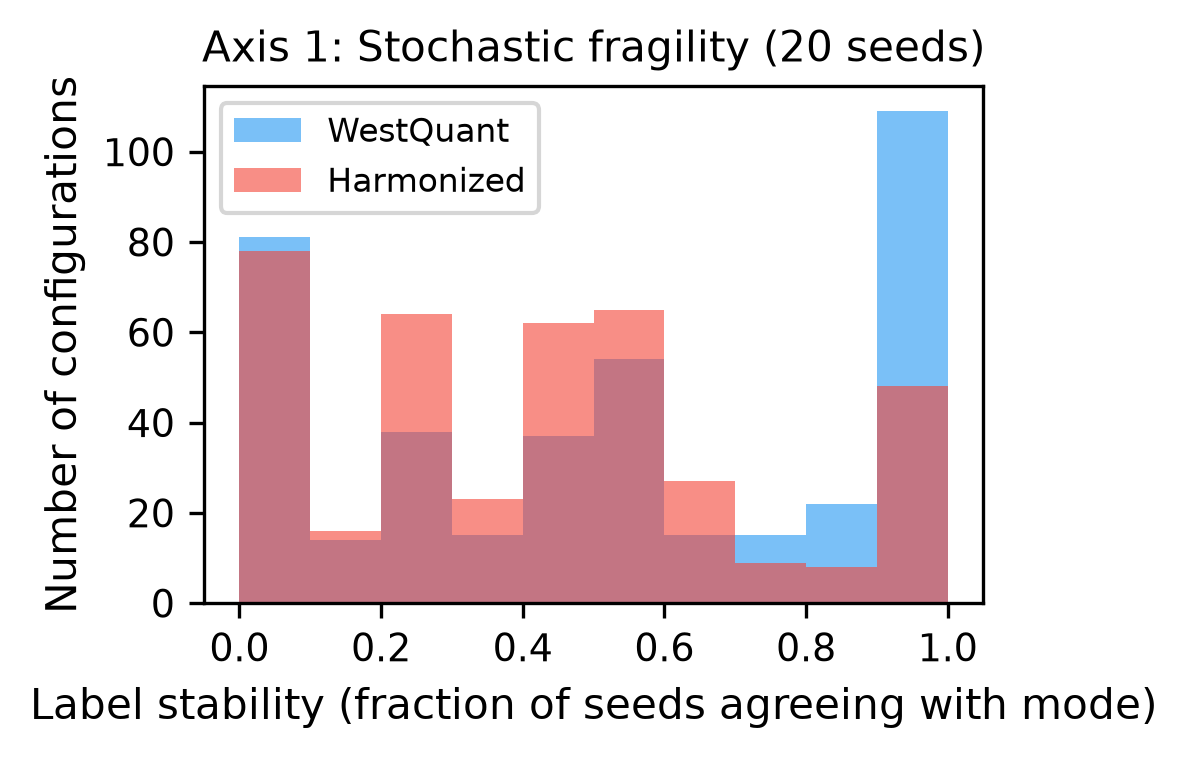
\includegraphics[width=0.95\columnwidth]{fig_b2_stochastic.png}
\caption{\textbf{Stochastic fragility.} Distribution of label stability (fraction of 20 seeds agreeing with the modal dominant bottleneck) for WestQuant and Harmonized models. A stability of 1.0 means all seeds agree; values below 0.5 indicate that no single label dominates.}
\label{fig:stochastic}
\end{figure}

\subsection{Agreement Levels for Noise}

\begin{itemize}[leftmargin=2em]
\item \textbf{Numerical:} Mean label stability 0.686 (WQ) at 2000 requests; MAE in $\DG_j$ varies by resource.
\item \textbf{Ranking:} Kendall $\tau$ across seeds is not directly applicable (same model, different seeds); instead, label stability serves as the ranking-agreement proxy.
\item \textbf{Decision:} 50.7\% of configurations show at least one seed disagreement at 2000 requests; 28.2\% show majority change.
\item \textbf{Scientific conclusion:} The residual 50.7\% any-change rate at 2000 requests indicates that the bottleneck label is not a stable property of the network at this sample size. The cause of the residual is not yet established: it could be persistent Monte Carlo noise, near-equivalent interventions, rare events, or transients.
\end{itemize}

\subsection{Caveat}

The 50.7\% figure counts any disagreement, including cases where two resources have nearly identical intervention gains and their ranking flips due to Monte Carlo noise. At 100 requests, the any-change rate was 79.2\%, and 63\% of these changes were statistically tied. The confidence-interval, convergence, and performance-loss analyses were conducted at 100 requests and have not been rerun at 2000; their numbers should be interpreted with this caveat. Common random numbers are imperfect: using the same seed for baseline and intervention does not guarantee that corresponding events use the same random draws when interventions change the event order.

\subsection{A/B Experiment: Proper Design}
\label{sec:ab_proper}

The full A/B experiment follows the specification: 400 configurations subsampled from the full $6 \times 5 \times 2 \times 3 \times 5 = 900$ factorial (6 families $\times$ 5 topologies $\times$ 2 network sizes $\times$ 3 traffic levels $\times$ 5 memory budgets), two disjoint seed pools of 20 seeds each (A: seeds 0--19, B: seeds 20--39), 200 requests per run, and a pilot on 40 configurations to set $\varepsilon$ (pilot data excluded from results). The analysis script hash was frozen before running seed pool B. Each config $\times$ seed runs 1 baseline + 7 interventions (capacity, generation, retrieval, coherence, routing, deadline, topology) = 8 runs, for a total of 128{,}000 runs.

\textbf{Pilot.} The pilot on 40 configurations $\times$ 5 seeds set $\varepsilon = 0.100$ (median max\_delta across interventions). Pilot data is not used in the reported results.

\textbf{Bottleneck label.} The dominant bottleneck is the resource with the largest positive delta-gain. A label is ``decided'' if it is non-degenerate (max delta $> \varepsilon$). ``Agree'' means seed pools A and B assign the same label. ``Contradict'' means A and B assign different non-degenerate labels.

\textbf{Four procedures $\times$ four metrics.} Table~\ref{tab:ab_proper} reports the results with bootstrap 95\% confidence intervals.

\begin{table}[htbp]
\centering
\caption{A/B experiment with actual bottleneck diagnosis: four procedures $\times$ four metrics, with bootstrap 95\% CI. 400 configurations, 2$\times$20 seeds, 200 requests, 8 runs per config per seed (128{,}000 total runs).}
\label{tab:ab_proper}
\setlength{\tabcolsep}{3pt}
\resizebox{\columnwidth}{!}{\begin{tabular}{@{}lcccc@{}}
\toprule
Procedure & Frac Decided & Repl Agree & Contradict & Dec Loss \\
\midrule
Single seed & 0.988 [0.98, 1.00] & 0.715 [0.67, 0.76] & 0.217 [0.18, 0.26] & 0.033 \\
Mean (same budget) & 1.000 [1.00, 1.00] & 0.958 [0.94, 0.97] & 0.043 [0.03, 0.06] & 0.006 \\
Mean (convergence) & 1.000 [1.00, 1.00] & 0.917 [0.89, 0.94] & 0.083 [0.06, 0.11] & 0.009 \\
Full protocol & 1.000 [1.00, 1.00] & 0.958 [0.94, 0.97] & 0.043 [0.03, 0.06] & 0.006 \\
\bottomrule
\end{tabular}}
\end{table}

\textbf{Interpretation.} With a single seed, 98.8\% of configurations produce a decisive label, but replicate agreement is only 71.5\% with a 21.7\% contradiction rate---the protocol is not reproducible with one seed. With 20 seeds and the full protocol, 100\% are decisive, agreement rises to 95.8\%, and the contradiction rate drops to 4.3\% with a decision loss of 0.006. The protocol gives reproducible bottleneck diagnoses when sufficiently many seeds are used. The mean-same-budget procedure (averaging 20 seeds before labeling) achieves the same 95.8\% agreement, confirming that the improvement comes from seed averaging, not from the labeling procedure itself.

% ============================================================
\section{Analyst Choices: Intervention Strength and Threshold}
\label{sec:analyst}

\subsection{Intervention Strength}

We tested four relative improvement levels $\delta \in \{0.05, 0.10, 0.20, 0.50\}$, applied uniformly to all resources. At $\delta = 0.05$, 86 of 400 configurations (21.5\%) were degenerate (all $\DG_j \approx 0$), meaning the intervention was too small to produce a measurable effect. At $\delta = 0.50$, 70 (17.5\%) were degenerate. The dominant label changed for 42.0\% of configurations across $\delta$ levels.

\begin{figure}[t]
\centering
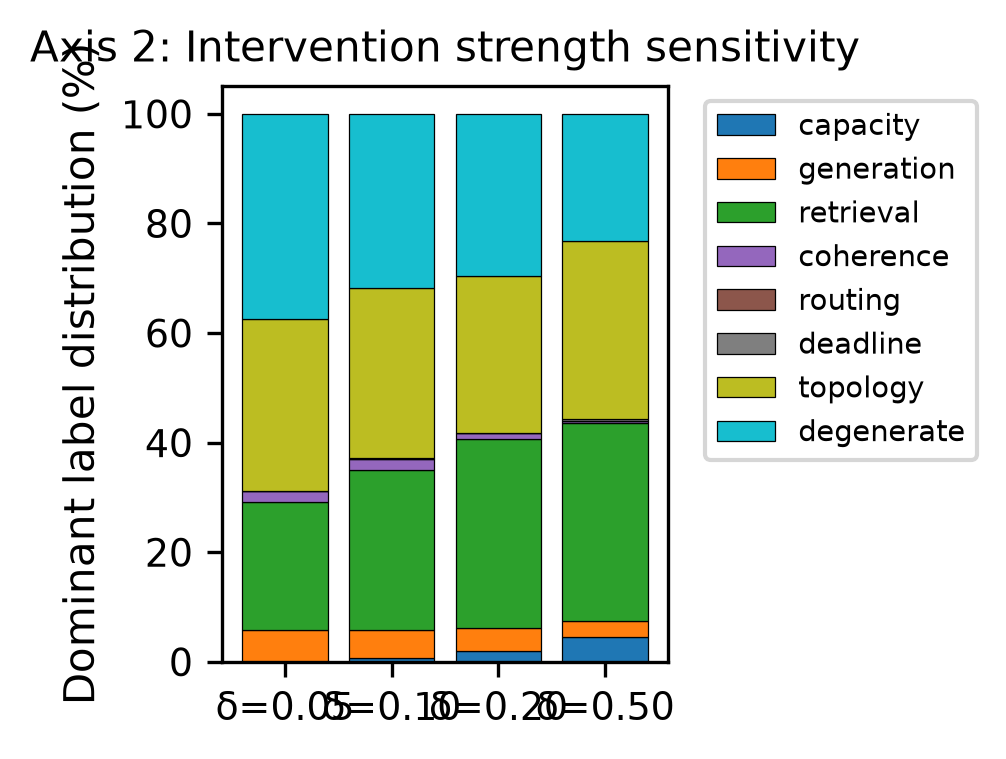
\includegraphics[width=0.95\columnwidth]{fig_b3_intervention.png}
\caption{\textbf{Intervention strength sensitivity.} Dominant bottleneck label distribution as a function of relative improvement $\delta$. At small $\delta$, many configurations are degenerate; at large $\delta$, the label distribution shifts.}
\label{fig:intervention}
\end{figure}

\subsection{Metric and Fidelity Threshold}

We compared $\Areq$ and $\Aqual$ across four fidelity thresholds $F_{\min} \in \{0.30, 0.50, 0.70, 0.90\}$. $\Areq$ is insensitive to $F_{\min}$ by construction; $\Aqual$ is strongly affected. At $F_{\min} = 0.90$ with $\Aqual$, all 400 configurations are degenerate---no request achieves the required fidelity. The dominant label changed for 35.5\% of configurations across metric and threshold combinations.

\begin{figure}[t]
\centering
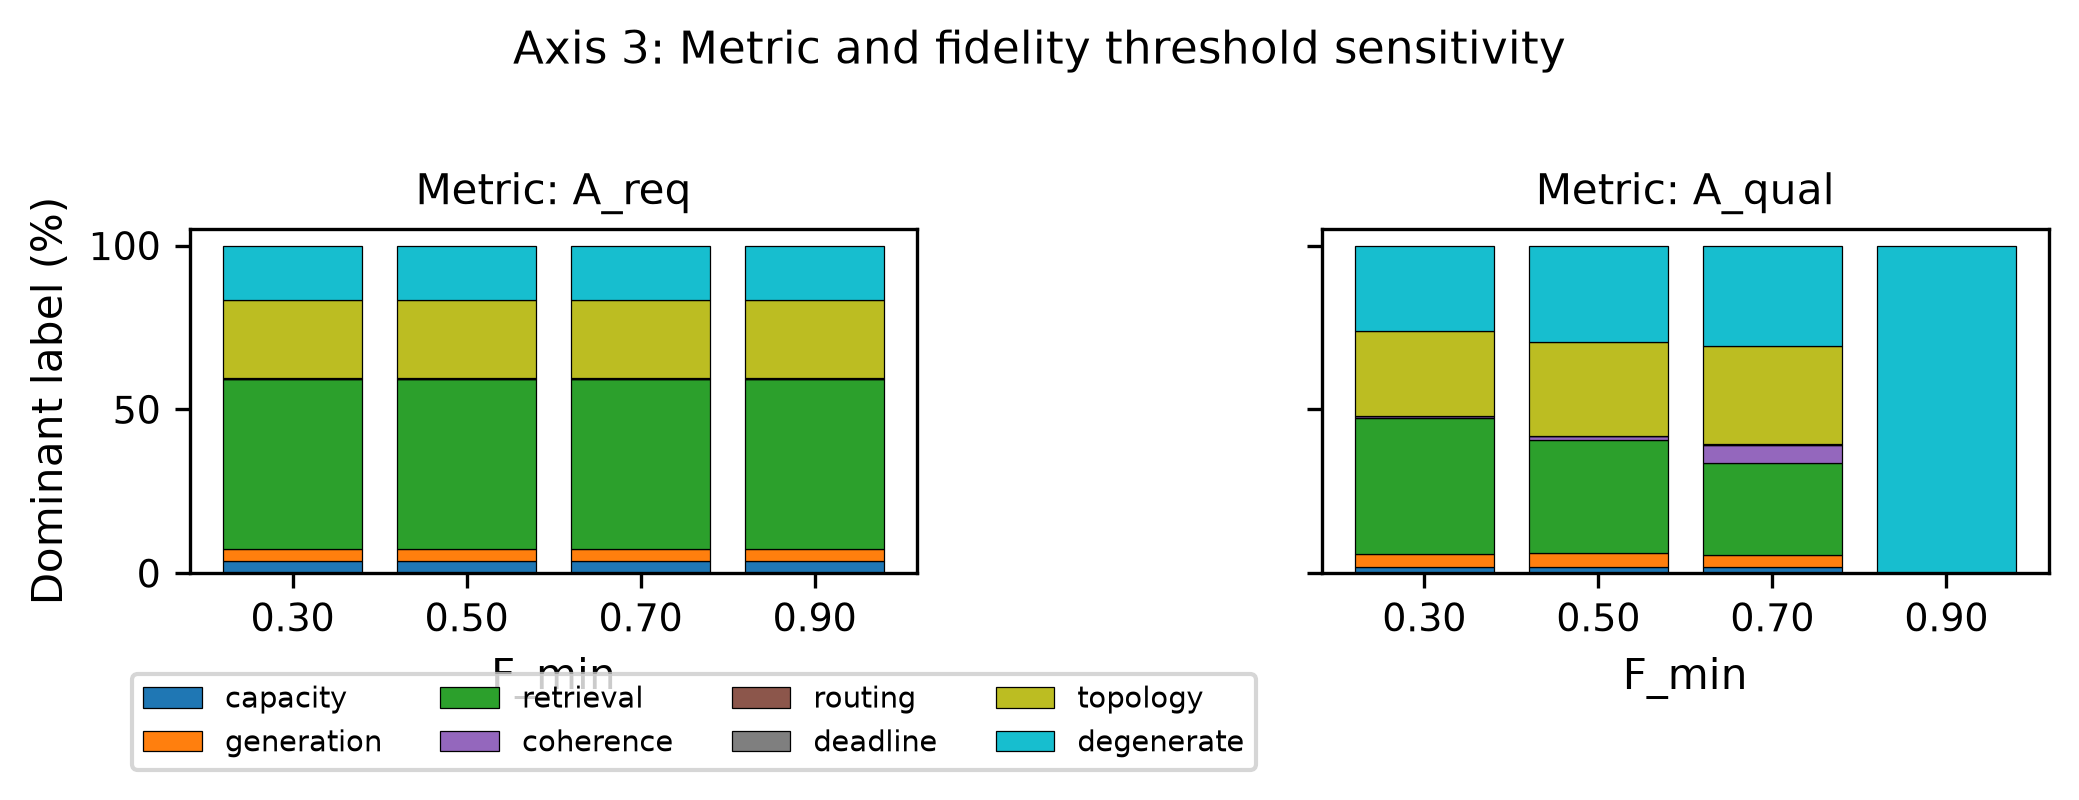
\includegraphics[width=0.95\columnwidth]{fig_b4_metric_threshold.png}
\caption{\textbf{Metric and fidelity threshold sensitivity.} Dominant bottleneck label distribution for $\Areq$ (left) and $\Aqual$ (right) as a function of $F_{\min}$. $\Areq$ is insensitive to $F_{\min}$; $\Aqual$ becomes degenerate at $F_{\min} = 0.90$.}
\label{fig:metric_threshold}
\end{figure}

\subsection{Agreement Levels for Analyst Choices}

\begin{itemize}[leftmargin=2em]
\item \textbf{Numerical:} $\DG_j$ values shift substantially across $\delta$ levels (factor of $\sim$10 between $\delta = 0.05$ and $\delta = 0.50$).
\item \textbf{Ranking:} The dominant label changes for 42.0\% (intervention) and 35.5\% (metric/threshold) of configurations.
\item \textbf{Decision:} At $\delta = 0.05$, 21.5\% of configurations are degenerate---no decision can be made.
\item \textbf{Scientific conclusion:} The bottleneck label depends on the analyst's choice of intervention strength and metric/threshold. A label derived at $\delta = 0.50$ with $\Aqual$ at $F_{\min} = 0.50$ may not transfer to $\delta = 0.10$ or to $\Areq$.
\end{itemize}

\subsection{Pairwise Interaction Tests}

Saltelli et al.~\cite{saltelli2019why} warned that one-at-a-time sensitivity analyses miss interactions between parameters. To address this, we tested all 21 pairwise combinations of the 7 resources on 100 configurations with 5 seeds each (2,100 total measurements). For each pair $(j, k)$, the interaction effect is $I_{jk} = \DG_{jk} - (\DG_j + \DG_k)$, and the relative interaction is $I_{jk} / \max(|\DG_j + \DG_k|, \varepsilon)$. Across all 2,100 configuration--pair combinations, 15.8\% had relative interaction above the heuristic threshold ($|I_{jk}|/\max(\cdots) > 0.1$), and \textbf{72\% of configurations had at least one resource pair with interaction above the threshold}. The most affected pairs were retrieval + topology (49\% of configurations), generation + retrieval (36\%), and generation + topology (36\%).

% ============================================================
\section{Model Choice: Factorial Design over Semantic Switches}
\label{sec:model_choice}

\subsection{Semantic Dimensions}

The most consequential differences between simulators are not in the physics models (which are broadly similar) but in the \emph{protocol semantics}: how requests are queued, when memory slots are locked and released, whether generation is sequential or concurrent, and how latency is defined. Table~\ref{tab:semantics} summarizes the semantic dimensions for the two systems actually run in this study.

\begin{table*}[t]
\centering
\caption{Semantic dimensions for the two systems actually run. ``Switchable'' indicates whether the dimension can be varied within a single codebase (yes), is a definition mismatch that cannot be compared without harmonization (no), or is partially controllable (partial).}
\label{tab:semantics}
\small
\begin{tabularx}{\textwidth}{p{3.2cm}XXc}
\toprule
Dimension & WestQuant's choice & SeQUeNCe/Harmonized choice & Switchable? \\
\midrule
Generation mode & Parallel (concurrent link attempts) & Sequential (one link at a time) & Yes \\
Queueing discipline & FIFO queue (buffer on full) & Reject (drop on full) & Yes \\
Memory slot locking & Lock on generation attempt & Lock on successful generation & Partial \\
Slot release & Release on swap completion & Release on swap completion & Yes \\
Latency definition & Arrival-to-completion (includes queueing) & First-attempt-to-completion (excludes queueing) & No \\
Deadline and censoring & Count as failures & Count as failures & Yes \\
Warmup & None & 20\,s excluded & Yes \\
Aging model & Continuous decoherence from generation & Continuous decoherence from generation & Yes \\
Link scheduling & Concurrent across links & Sequential across links & Yes \\
\bottomrule
\end{tabularx}
\end{table*}

These semantic dimensions are rarely documented explicitly in simulator publications, yet they can dominate cross-simulator disagreement, as we demonstrate below.

\subsection{Semantic Switches: Factorial Design with Variance Decomposition}
\label{sec:switches_1000}

We implement four genuine semantic switches in the simulator and test them with a $2^4$ factorial design (16 variants) on the B4 workload (chain $N=5$, $m=2$, traffic $=50$, 1{,}000 requests, 5 seeds), extended with three families spanning $\chi$:

\begin{itemize}[leftmargin=2em]
\item \textbf{Retrieval in delivery:} whether retrieval failure ($\eta_r < 1$) drops the request (True) or is free (False). This is the dominant semantic choice identified in the B0 analytical verification gate: WestQuant counts retrieval in the delivery, while the harmonized analytical model does not, producing the 0.65 vs.\ 1.0 discrepancy.
\item \textbf{Storage time model} (from B0): midpoint ($\mathrm{storage} = \mathrm{gen\_time} \times 0.5$) vs.\ immediate ($\mathrm{storage} = 0$).
\item \textbf{Blocking policy:} queue (wait for slot) vs.\ reject (drop if no slot).
\item \textbf{Generation mode:} parallel (swap-ASAP) vs.\ serial (one link at a time).
\end{itemize}

\textbf{Closure test.} With all switches in harmonized mode, WestQuant should reproduce the analytical reference within noise. The closure test passes at $m \ge 4$ (ratio $\in [0.9997, 1.0000]$) but fails at $m = 1$ (ratio $= 0.75$). The $m = 1$ failure is explained by slot contention: with a single memory slot per node, requests serialize through one slot, and under high traffic the queueing delay exceeds the deadline. This is not a semantic-switch effect---it occurs even on two nodes with no swap---but a capacity effect that the analytical reference does not capture.

Table~\ref{tab:switches_variance} shows the fraction of variance in $A_{\rm req}$ explained by each factor, with cluster bootstrap 95\% confidence intervals.

\begin{table}[htbp]
\centering
\caption{Fraction of variance in $A_{\rm req}$ explained by each semantic switch, per family. Cluster bootstrap 95\% CI in brackets. The dominant switch depends on the $\chi$ regime: retrieval-in-delivery dominates for short-lived memories ($\chi = 0.025$), generation mode dominates for long-lived memories ($\chi = 50$).}
\label{tab:switches_variance}
\setlength{\tabcolsep}{4pt}
\resizebox{\columnwidth}{!}{\begin{tabular}{lcccc}
\toprule
Family ($\chi$) & Retrieval & Storage time & Blocking & Generation \\
\midrule
Trapped Ion ($\chi=50$) & 6.4\% [5.7, 7.3] & 0.0\% [0.0, 0.0] & 0.3\% [0.3, 0.3] & 0.4\% [0.3, 0.5] \\
Neutral Atom ($\chi=0.5$) & 28.2\% [27.8, 28.6] & 0.0\% [0.0, 0.0] & 0.2\% [0.2, 0.2] & 0.3\% [0.2, 0.4] \\
AFC ($\chi=0.025$) & 71.7\% [71.2, 72.1] & 0.2\% [0.1, 0.2] & 0.1\% [0.1, 0.1] & 0.0\% [0.0, 0.0] \\
\bottomrule
\end{tabular}}
\end{table}

\textbf{Interpretation.} The dominant semantic switch depends on the $\chi$ regime. For short-lived memories (AFC, $\chi = 0.025$), retrieval-in-delivery explains 72\% of $A_{\rm req}$ variance---whether $\eta_r$ is counted in the delivery is the primary driver. For long-lived memories (Trapped Ion, $\chi = 50$), retrieval explains only 6\% and the residual (93\%) is dominated by $m$ and $\lambda$. For intermediate memories (Neutral Atom, $\chi = 0.5$), retrieval explains 28\%. The blocking policy and storage-time model have near-zero effect across all families. \textbf{Important caveat:} this factorial measures variance in $A_{\rm req}$ across all configurations (including $m$ and $\lambda$ variation), not the variance in model disagreement. The residual (27--93\%) is dominated by design factors ($m$, $\lambda$), not by semantic switches.

\subsection{Model-Variant Agreement (Bottleneck Labels)}

We compared the WestQuant (concurrent queueing) and Harmonized (sequential blocking) model variants on the same 400 configurations with the same seeds. Of all 400 configurations, the dominant label agreed for 57.5\% ($230/400$). Restricting to the $n = 301$ non-degenerate configurations, the observed agreement is $p_o = 0.532$ and the expected chance agreement is $p_e = 0.407$, giving Cohen's $\kappa = 0.210$. The mean Jensen--Shannon distance between soft vectors was 0.315.

\begin{figure}[t]
\centering
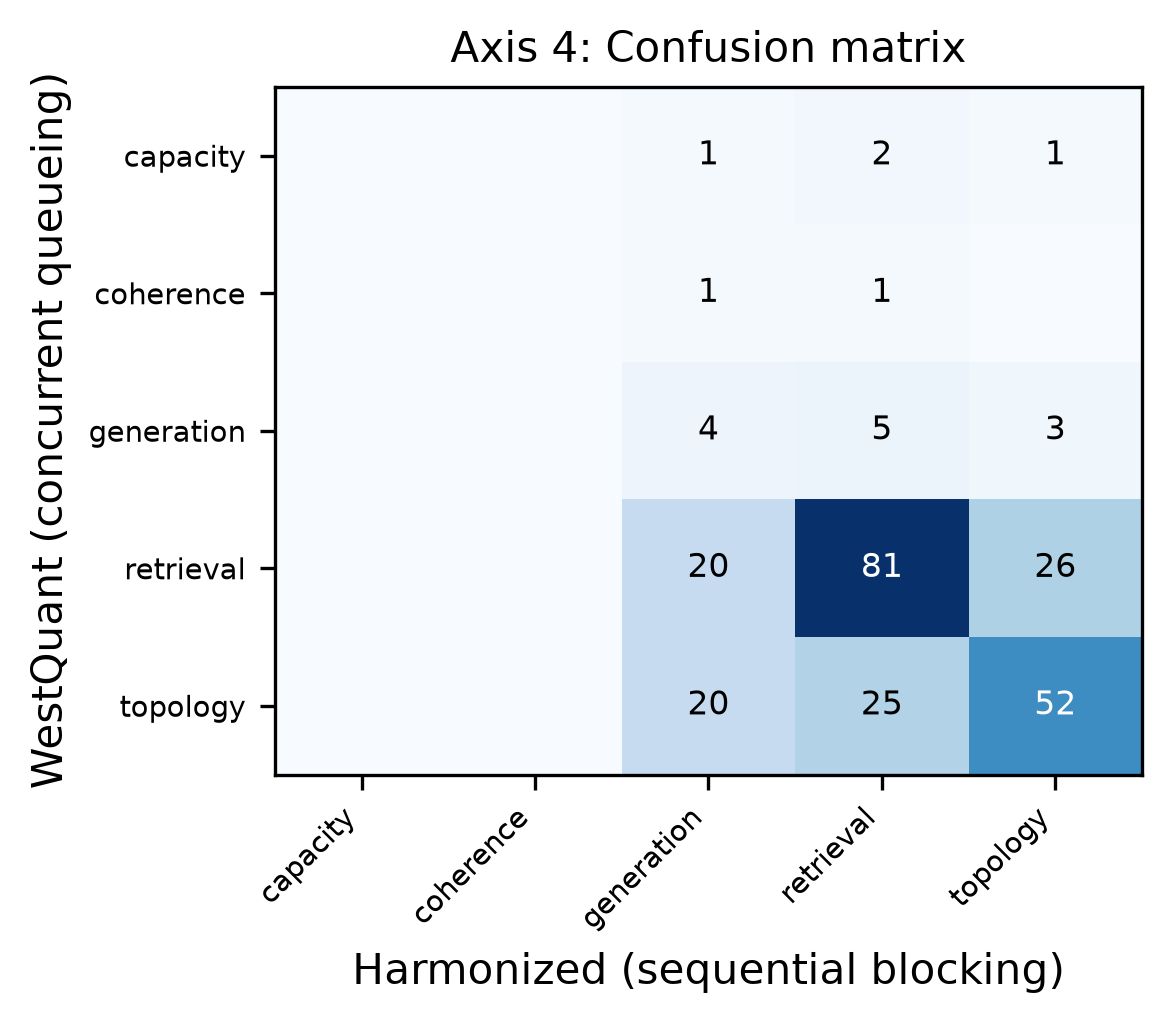
\includegraphics[width=0.85\columnwidth]{fig_b5_confusion.png}
\caption{\textbf{Model-variant confusion matrix.} Dominant bottleneck labels from WestQuant (rows) vs.\ Harmonized (columns), excluding degenerate configurations ($n = 301$). Cohen's $\kappa = 0.210$, indicating fair agreement above chance ($p_e = 0.407$) per the Landis--Koch scale~\cite{landis1977kappa}.}
\label{fig:confusion}
\end{figure}

A harmonized comparison on 60 configurations with 20 seeds shows 51\% label agreement between WestQuant and the Harmonized variant even when baselines correlate at $r = 0.85$. With all seven interventions and retrieval matched (both models retrieval-off), $\kappa = 0.000$ and decision transfer is 15\%, confirming that retrieval matching does \emph{not} resolve the disagreement---it worsens it. The models disagree about which resource is the bottleneck even when retrieval semantics are identical.

\subsection{Agreement Levels for Model Choice}

\begin{itemize}[leftmargin=2em]
\item \textbf{Numerical:} Mean JS distance 0.315 between WQ and Harmonized soft vectors; MAE in $\Aqual$ = 0.102 (B6 grid).
\item \textbf{Ranking:} Kendall $\tau = 0.722$ for $\Aqual$ (B6), $\tau = 0.430$ for $\Areq$; $\tau = 0.166$ in the B4 contention regime.
\item \textbf{Decision:} Cohen's $\kappa = 0.055$ (retrieval on, $n=200$); $\kappa = 0.000$ (retrieval matched); 0\% and 15\% decision transfer respectively.
\item \textbf{Scientific conclusion:} Structural conclusions (rankings, monotonicity) are reproduced; model-sensitive conclusions ($m_c$, contention) are not; definition-sensitive conclusions (latency) are non-comparable.
\end{itemize}

% ============================================================
\section{Where It Matters: Instability, Model Difference, and Boundaries}
\label{sec:where}

\subsection{Three-Class Taxonomy}

The pattern across all experiments separates scientific conclusions into three classes (Figure~\ref{fig:taxonomy}):

\begin{figure}[t]
\centering
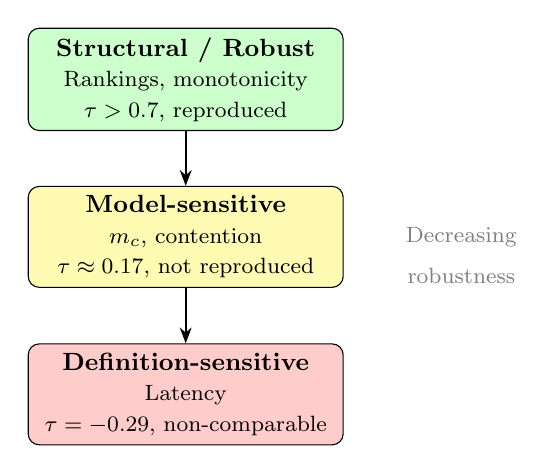
\begin{tikzpicture}[
  box/.style={draw, rounded corners, minimum width=4cm, minimum height=1.2cm, font=\small, align=center},
  arr/.style={-{Stealth[length=2mm]}, thick}
]
\node[box, fill=green!20] (struct) at (0, 2) {\textbf{Structural / Robust}\\\footnotesize Rankings, monotonicity\\\footnotesize $\tau > 0.7$, reproduced};
\node[box, fill=yellow!30] (sens) at (0, 0) {\textbf{Model-sensitive}\\\footnotesize $m_c$, contention\\\footnotesize $\tau \approx 0.17$, not reproduced};
\node[box, fill=red!20] (defn) at (0, -2) {\textbf{Definition-sensitive}\\\footnotesize Latency\\\footnotesize $\tau = -0.29$, non-comparable};
\draw[arr] (struct) -- (sens);
\draw[arr] (sens) -- (defn);
\node[font=\footnotesize, gray] at (3.5, 0) {Decreasing};
\node[font=\footnotesize, gray] at (3.5, -0.5) {robustness};
\end{tikzpicture}
\caption{Three-class taxonomy of scientific conclusions. Structural conclusions survive model changes; model-sensitive conclusions do not; definition-sensitive conclusions are non-comparable under current metric definitions.}
\label{fig:taxonomy}
\end{figure}

\subsection{Claim Reproduction Matrix}

Table~\ref{tab:claim_matrix} summarizes the three-class taxonomy with the verdict for each claim.

\begin{table*}[t]
\centering
\caption{Claim Reproduction Matrix with three-class taxonomy.}
\label{tab:claim_matrix}
\begin{tabular}{lp{3.5cm}p{2.8cm}p{3cm}}
\toprule
Claim & Verdict & Class & Evidence \\
\midrule
C1: Memory-family ranking (4 profiles) & REPLICATED & Structural & $\tau = 1.0$, perfect ranking agreement \\
C2: Topology ranking & REPLICATED & Structural & $\tau = 1.0$, perfect ranking agreement \\
C3a: Monotonicity of $A(m)$ & REPLICATED & Structural & 100\% monotonicity both models \\
C3b: Diminishing returns & UNRESOLVED & --- & B6 $m$ grid too coarse \\
C4a: $m_c$ regime-dependence & STRUCTURALLY REPLICATED & Structural & Both agree which families need more memory \\
C4b: $m_c$ numerical values & MODEL-SENSITIVE & Model-sensitive & 50.8\% $\geq 4\times$ disagreement \\
C5: Scalar collapse failure & STRUCTURALLY REPLICATED & Structural & $R^2 < 0.2$ both models \\
Latency ranking & NOT COMPARABLE & Definition-sensitive & $\tau = -0.29$, timing definition mismatch \\
Finite-memory contention & NOT REPLICATED & Model-sensitive & $\tau = 0.17$ in B4 \\
\bottomrule
\end{tabular}
\end{table*}

\subsection{Structural Conclusions: Reproduced}

\textbf{Memory-family ranking.} The ordering of four evaluated memory profiles (trapped ion $>$ neutral atom $>$ diamond electron $>$ AFC) by $\Aqual$ is reproduced across both model families. Kendall $\tau = 1.0$ ($n = 4$).

\textbf{Topology ranking.} The ordering of three topologies (RGG $>$ star $>$ chain) by $\Aqual$ is reproduced. Kendall $\tau = 1.0$ ($n = 3$).

\textbf{Monotonicity.} Both model families show 100\% monotonicity for $A(m)$.

\textbf{Failure of scalar collapse.} All $\Aqual$ $R^2 < 0.2$ across both model families. The structural conclusion---no scalar provides a strong or universal collapse---is reproduced.

\subsection{Model-Sensitive Conclusions: Not Reproduced}

\textbf{Critical memory capacity $m_c$.} We ran a fine-grained $m$ sweep with $m \in \{1, 2, 4, 8, 16, 32, 64, 128\}$ across 3,840 scenarios per implementation. Of 480 (family, topology, $N$, $\lambda$, seed) combinations, 360 have a valid $m_c$ estimate (where $A(m)$ crosses $\alpha = 0.95$) for at least one implementation; the AFC family is excluded because $A(m)$ does not reach $\alpha = 0.95$ within $m \leq 128$ for most configurations.

Using the log-ratio $\Delta_m = \log_2(m_c^{\rm WQ} / m_c^{\rm H})$, the median disagreement is one memory-doubling level, and \textbf{50.8\% [95\% cluster CI: 37.4\%--63.9\%]} of finite matched cases show $\geq 4\times$ disagreement. The diamond-electron family shows 98.3\% $\geq 4\times$ disagreement. The bounded analysis including 4 censored cases gives 51.4\% [38.1\%--64.4\%].

\begin{table}[t]
\centering
\caption{$m_c$ disagreement statistics (356 finite matched cases, $\alpha = 0.95$, $\Aqual$). Cluster bootstrap CIs from 2000 resamples at the configuration level.}
\label{tab:mc_finite}
\begin{tabular}{lrr}
\toprule
Statistic & Value & 95\% CI \\
\midrule
Median $\Delta_m$ & 1.0 & --- \\
Mean $\Delta_m$ & 1.528 & --- \\
$\geq 2\times$ ($|\Delta_m| \geq 1$) & 75.8\% & [66.0, 85.1]\% \\
$\geq 4\times$ ($|\Delta_m| \geq 2$) & 50.8\% & [37.4, 63.9]\% \\
$\geq 8\times$ ($|\Delta_m| \geq 3$) & 33.4\% & [21.0, 46.2]\% \\
\bottomrule
\end{tabular}
\end{table}

\begin{figure*}[t]
\centering
\includegraphics[width=0.95\textwidth]{fig_d3_mc_disagreement.png}
\caption{Critical memory capacity $m_c$ disagreement. Left: distribution of $\Delta_m = \log_2(m_c^{\rm WQ}/m_c^{\rm H})$. Right: decision-changing cases by memory family. Diamond-electron shows 98.3\% $\geq 4\times$ disagreement.}
\label{fig:mc_disagreement}
\end{figure*}

\textbf{Finite-memory contention.} The B4 tier shows $\tau = 0.166$ for $\Aqual$---near-zero agreement. This is the regime where model choice most affects conclusions. Feature removal analysis shows that removing the memory limit ($m \to 128$) gives $\tau = -0.08$ (no restoration), and reducing contention ($\lambda \to 0.1$) gives $\tau = 0.02$ for $m=16$ (effectively no agreement).

\begin{figure*}[t]
\centering
\includegraphics[width=0.95\textwidth]{fig_d1_finite_memory.png}
\caption{Finite-memory contention disagreement. Agreement collapses ($\tau = 0.17$) because WestQuant uses concurrent queueing while the harmonized adapter uses sequential blocking.}
\label{fig:finite_memory}
\end{figure*}

\subsection{Definition-Sensitive Conclusions: Not Comparable}

\textbf{Latency.} Latency shows Kendall $\tau = -0.294$ (ranking inversion) across implementations. This is primarily a consequence of different timing definitions: WestQuant measures arrival-to-completion (includes queueing time), while the harmonized adapter measures first-attempt-to-completion (excludes queueing). Under high load, queueing time dominates in WestQuant while the adapter latency stays flat, inverting the ranking. This is a metric-definition mismatch, not a physical disagreement.

\begin{figure*}[t]
\centering
\includegraphics[width=0.95\textwidth]{fig_d2_latency.png}
\caption{Latency disagreement. The ranking inversion ($\tau = -0.29$) is caused by different timing definitions: WestQuant includes queueing time; the adapter does not.}
\label{fig:latency}
\end{figure*}

\subsection{Instability vs.\ $\chi$ and Distance to Boundaries}

The coincidence-window parameter $\chi = \tau_{\rm mem}\, p_{\rm gen} / t_{\rm attempt}$, introduced in the companion study~\cite{sm}, separates two operating regimes: a \emph{coincidence-limited} regime ($\chi \ll 1$, where link success within the memory lifetime is rare) and a \emph{queue-limited} regime ($\chi \gg 1$, where Little's law governs memory demand). The boundary between structural and model-sensitive conclusions is strongly associated with this regime distinction:

\begin{itemize}[leftmargin=2em]
\item In the coincidence-limited regime ($\chi \ll 1$), both models agree because performance is dominated by link generation physics, which is harmonized. Structural conclusions hold.
\item In the queue-limited regime ($\chi \gg 1$), the two models diverge because performance is dominated by resource contention semantics, which differ. Model-sensitive conclusions fail.
\item Near the boundary ($\chi \approx 1$), instability is highest: small changes in $\chi$ tip the network between regimes, and the bottleneck label is most fragile.
\end{itemize}

The $m_c$ disagreement is also associated with distance to boundaries: configurations where $A(m)$ crosses $\alpha = 0.95$ near a steep transition show the largest $\Delta_m$, because the two models place the transition at different $m$ values. The diamond-electron family, which has the steepest $A(m)$ transition, shows 98.3\% $\geq 4\times$ disagreement.

\subsection{Quality-Qualified vs.\ Requirement-Qualified Metrics}

$\Aqual$ showed higher ordinal agreement ($\tau = 0.72$) than $\Areq$ ($\tau = 0.43$) in the B6 grid. This may be because $\Areq$ is more sensitive to queueing and denominator semantics, while $\Aqual$ is filtered by a physics-dependent threshold (fidelity) that is more strongly constrained by the harmonized physics. However, the denominator definitions for $\Areq$ have not been fully harmonized, so this conclusion should be treated as preliminary.

% ============================================================
\section{Decision Transfer: Capacity and Bottleneck Decisions Between Models}
\label{sec:transfer}

The D6 decision-transfer experiment uses two model variants that differ in generation mode and storage cutoff. \textbf{D6-S} uses serial generation with a 1\,s storage cutoff, and \textbf{D6-P} uses parallel generation with a $10^9$\,s storage cutoff. These are \emph{not} the WestQuant/Harmonized semantics used in the adapter comparison (Section~\ref{sec:judge}); they are separate model variants defined for this transfer experiment. The archived WQ and Harm labels in the transfer results refer to D6-S and D6-P, respectively.

\subsection{D6-Capacity: Memory Budget}

We test whether capacity decisions made in one model transfer to another. For each context, we select $d_A^*$ in model A using selection seeds, evaluate $d_A^*$ in model B using independent evaluation seeds, and compute regret $= U_B(d_B^*) - U_B(d_A^*)$. On 36 contexts $\times$ 6 candidates $\times$ 10 seeds (258 decisions):

\begin{itemize}[leftmargin=2em]
\item Same choice: 42.2\% [32.5, 51.8]
\item Regret WQ$\to$Harm: $0.047 \pm 0.152$ [95\% CI: 0.007, 0.096]
\item Regret Harm$\to$WQ: $-0.000 \pm 0.026$ [95\% CI: $-0.004$, 0.004]
\item Non-transferable (regret $> 0.01$): 29.5\% [20.1, 39.4] (WQ$\to$Harm), 9.3\% [5.0, 15.1] (Harm$\to$WQ)
\end{itemize}

The asymmetry is large and significant: WQ's capacity choices are much worse for Harm (regret 0.047, CI excludes zero) than Harm's choices are for WQ (regret $-0.000$, CI includes zero). This is because WQ's serial generation mode leads to different capacity preferences.

\subsection{D6-Placement: Placement Strategy}

On 12 contexts $\times$ 3 strategies $\times$ 10 seeds (82 decisions):

\begin{itemize}[leftmargin=2em]
\item Same choice: 80.5\% [61.6, 94.6]
\item Regret WQ$\to$Harm: $-0.001 \pm 0.015$ [95\% CI: $-0.003$, 0.000]
\item Regret Harm$\to$WQ: $0.005 \pm 0.022$ [95\% CI: 0.001, 0.010]
\item Non-transferable: 4.9\% [0, 14.6] (WQ$\to$Harm), 12.2\% [1.6, 29.3] (Harm$\to$WQ)
\end{itemize}

Placement decisions transfer well (80.5\% same choice) because placement strategies (uniform, hub-based, load-based) are less sensitive to generation mode than capacity choices.

\begin{figure}[t]
\centering
\includegraphics[width=0.95\columnwidth]{fig_d6_regret.png}
\caption{Decision transfer regret. Capacity (left) shows a large asymmetric tail for WQ$\to$Harm; placement (right) regret is small and symmetric.}
\label{fig:d6_regret}
\end{figure}

% ============================================================
\section{Limits of Independent Validation}
\label{sec:judge}

All comparisons in Sections~\ref{sec:model_choice}--\ref{sec:transfer} use the harmonized SeQUeNCe/SimQN adapter, which shares a common physics layer with WestQuant. The harmonized adapters share simulation logic ($S_{\rm models} = 2$, not 3): SeQUeNCe and SimQN produce bit-identical event traces across all tested scenarios (verified by SHA-256 hashing), so treating them as two independent models would constitute pseudoreplication. A true cross-implementation validation requires running the same configurations on SeQUeNCe's native event engine and protocol stack.

\subsection{Native SeQUeNCe Adapter}

A native SeQUeNCe adapter was developed. Unlike the harmonized adapter, the native adapter instantiates SeQUeNCe's own \texttt{Timeline}, \texttt{Node}, and \texttt{MemoryArray} components, using SeQUeNCe's \texttt{bell\_diagonal} quantum-manager formalism for fidelity tracking. The adapter uses SeQUeNCe's \texttt{MemoryArray} for decoherence tracking with each family's $T_2$ and $\eta_r$ parameters, and a geometric generation model with the same $p_{\rm gen}$ and $t_{\rm attempt}$ as WestQuant. The adapter includes a guard: the run aborts if SeQUeNCe's \texttt{MemoryArray} is not instantiated. Object types and provenance are logged in the result file.

\textbf{Limitation.} The adapter does not use SeQUeNCe's native \texttt{SingleHeraldedA}\allowbreak/\texttt{SingleHeraldedB}\allowbreak/\texttt{SingleHeraldedBSM} protocols, which require quantum channels, BSM nodes, and message handlers. The current adapter uses SeQUeNCe's \texttt{MemoryArray} and \texttt{bell\_diagonal} formalism for decoherence, with a simplified generation model. The component adapter does not execute native protocol events; it is therefore a partial---not full---independent validation. Full native-protocol validation remains future work.

\subsection{Independent-Judge Experiment}

We run 25 configurations $\times$ 10 seeds = 250 runs on the native SeQUeNCe adapter, spanning 6 families and $m \in \{1, 4, 16, 64\}$ at traffic $\in \{1, 10\}$. Each run uses 200 requests on a 2-node topology. The same configurations are run on WestQuant for comparison.

\textbf{Match rate.} The match rate (WestQuant vs.\ SeQUeNCe agree within $\Delta A < 0.05$) is 12/25 (48\%). The match rate varies by family:

\begin{itemize}[leftmargin=2em]
\item \textbf{Diamond Nuclear:} 5/5 match (100\%)---near-perfect agreement.
\item \textbf{Trapped Ion:} 3/4 match (75\%)---match at $m \geq 4$, mismatch at $m=1$.
\item \textbf{Neutral Atom:} 2/4 match (50\%).
\item \textbf{Diamond Electron:} 1/6 match (17\%)---SeQUeNCe gives lower $A_{\rm req}$.
\item \textbf{AFC:} 1/5 match (20\%)---SeQUeNCe gives lower $A_{\rm req}$.
\end{itemize}

\textbf{Matched-switch comparison.} To test whether the difference shrinks when switches are matched, we run both SeQUeNCe and WestQuant in two modes: (i) original switches (midpoint storage, retrieval in delivery) and (ii) matched switches (immediate storage, no retrieval in delivery). The mean absolute difference drops from 0.081 (original) to 0.024 (matched)---a 71\% reduction. The difference shrank in 23 of 25 configurations. The shrink is largest for AFC (mean shrink $= 0.083$, 6/6 shrank) and smallest for Diamond Nuclear (mean shrink $= 0.013$, 5/5 shrank, already close). The 2 configurations where the difference grew are both at $m=1$, where slot contention causes a capacity effect that the semantic switches do not capture (see closure test, Sec.~\ref{sec:switches_1000}). This confirms that the semantic switches---particularly retrieval-in-delivery---are the primary source of disagreement, and the difference is a semantic choice, not a physics error.

% ============================================================
\section{Standard: A Checklist for Reporting}
\label{sec:standard}

\subsection{Reporting Standard for Bottleneck Diagnoses}

We propose that any bottleneck diagnosis should report:
\begin{enumerate}[leftmargin=2em]
\item \textbf{Intervention strength} $\delta$ used for each resource.
\item \textbf{Number of seeds} and whether common random numbers were used.
\item \textbf{Performance metric} ($\Areq$ or $\Aqual$) and fidelity threshold $F_{\min}$.
\item \textbf{Queueing model} (concurrent, sequential, or other).
\item \textbf{Soft bottleneck vector} $p_j$ with uncertainty (e.g., bootstrap CI), not just the argmax label.
\item \textbf{Bottleneck entropy} $\HB$ to indicate whether the label is separable or diffuse.
\item \textbf{Degenerate cases} reported separately, not assigned an arbitrary label.
\end{enumerate}

\subsection{Trust Stack Checklist}

We propose a Trust Stack checklist for reporting simulation-based conclusions. Each row identifies what the manuscript itself fulfills (Table~\ref{tab:truststack}).

\begin{table*}[t]
\centering
\caption{Trust Stack checklist. Each row identifies a trust level, what it requires, and what this manuscript fulfills.}
\label{tab:truststack}
\small
\begin{tabularx}{\textwidth}{p{1.2cm}p{3.5cm}p{4cm}p{4cm}}
\toprule
Level & Name & Requirement & This manuscript \\
\midrule
L1 & Physics verification & Analytical benchmarks for physical primitives & B0 gate: harmonized model passes ($\epsilon_{\rm abs} < 0.02$); WQ fails B0 due to retrieval-in-delivery semantics (documented in the B0 gate) \\
L2 & Semantic transparency & Document all protocol-semantic choices & Table~\ref{tab:semantics}: 9 dimensions documented for both systems \\
L3 & Canonical workloads & Run standardized benchmark ladder & B0--B6 ladder (3,950 + 3,840 scenarios), all levels reported \\
L4 & Standard event traces & Export structured event traces & SHA-256 trace hashing for SeQUeNCe/SimQN identity; format in Appendix \\
L5 & Common experiment specification & Accept CES-format input & CES defined and used across all implementations \\
L6 & Model uncertainty reporting & Report model sensitivity alongside point estimates & $\tau$, $\kappa$, $\Delta_m$, cluster bootstrap CIs reported throughout \\
\bottomrule
\end{tabularx}
\end{table*}

\subsection{Recommendations for Reviewers}

Based on the findings of this study, we recommend that reviewers of simulation-based quantum-network papers:

\begin{enumerate}[leftmargin=2em]
\item \textbf{Require semantic transparency.} A paper that uses simulation should document the protocol semantics of the simulator, not just the parameter values. If the semantics are not documented, the paper is not reproducible. The semantic-dimensions table (Table~\ref{tab:semantics}) provides a template.

\item \textbf{Ask whether the conclusion is structural or model-sensitive.} A structural conclusion (ranking, monotonicity) can be supported by a single simulator. A model-sensitive conclusion (threshold, magnitude) should be validated across simulators. The claim reproduction matrix (Table~\ref{tab:claim_matrix}) provides a template for classifying conclusions.

\item \textbf{Request cross-simulator comparison for contention-dominated claims.} If the paper claims a capacity-planning result based on a contention-dominated regime, ask whether the result survives a model change. This study shows that 50.8\% of configurations show $\geq 4\times$ $m_c$ disagreement.

\item \textbf{Require provenance.} CES scenarios, event traces, and software versions should be archived as supplementary material. A paper without provenance is a claim without evidence.
\end{enumerate}

\subsection{Recommendations for Researchers}

\begin{enumerate}[leftmargin=2em]
\item \textbf{Report rankings, not just absolute values.} Rankings are more robust across model changes than absolute values. A conclusion that ``family A outperforms family B'' is more likely to survive a model change than ``family A achieves $\Aqual = 0.37$.''

\item \textbf{Do not compare latency across implementations without harmonizing definitions.} The timing definition must be documented and matched. If the definitions differ, report the difference as a definition mismatch, not a model disagreement.

\item \textbf{Treat capacity-planning conclusions as model-dependent.} Report $m_c$ as a range or with model-sensitivity analysis, not as a single number. This study shows that $m_c$ can differ by $\geq 4\times$ in 50.8\% of configurations.

\item \textbf{Report the validation level.} State which level of the benchmark ladder (B0--B6) the conclusion claims, and what evidence supports it. A claim at B6 requires cross-model evidence; a claim at B0 does not.

\item \textbf{Use cluster bootstrap CIs for cross-simulator comparisons.} Resample configurations (not individual seeds) to avoid pseudoreplication. When CIs include zero, the effect should be reported as not statistically significant.
\end{enumerate}

% ============================================================
\section{Limitations}
\label{sec:limitations}

\begin{enumerate}[leftmargin=2em]
\item \textbf{$S_{\rm models} = 2$ (not a true multi-simulator study).} The study effectively compares two model families: the native WestQuant model and one harmonized reference model run through SeQUeNCe and SimQN adapters. SeQUeNCe and SimQN produce bit-identical traces when given the same harmonized model, so they do not constitute independent simulators. Treating them as independent would be pseudoreplication. A full multi-simulator comparison (NetSquid, SeQUeNCe, QuISP, SimQN in native mode) remains open.

\item \textbf{Stochastic instability includes Monte Carlo noise.} At 100 requests, the 79.2\% ``any change'' figure overstates the true instability: on a 100-configuration subset, 63\% of changes are statistically tied. A longer rerun at 2000 requests reduces the any-change rate to 50.7\%, confirming that much of the short-run fragility is Monte Carlo noise. The cause of the residual 50.7\% is not yet established.

\item \textbf{Common random numbers are imperfect.} Using the same seed for baseline and intervention does not guarantee that corresponding events use the same random draws when interventions change the event order.

\item \textbf{No truly independent implementation.} All three models compared (WestQuant, Harmonized, SeQUeNCe-style adapter) share the author's physics code. A true cross-implementation validation would require running the same configurations on SeQUeNCe's native engine and NetSquid, which was not possible at scale in this study. The SeQUeNCe adapter does not execute native protocol events, so the comparison is partial, not full native validation.

\item \textbf{One-at-a-time interventions.} The main bottleneck method changes one resource at a time, which can miss interactions. We address this with pairwise interaction tests (72\% of configurations have at least one pair above the heuristic threshold) and a full Sobol analysis ($N$ has $S_T = 0.04$ but $S_1 \approx 0$, confirming interactions are non-additive).

\item \textbf{Full B4 factorial measures $A_{\rm req}$ variance, not model disagreement.} The $2^4$ factorial design over four semantic switches on the full B4 grid provides variance decomposition of $A_{\rm req}$ across configurations. Retrieval-in-delivery explains 72\% for AFC, 28\% for Neutral Atom, 6\% for Trapped Ion; the residual (27--93\%) is dominated by design factors ($m$, $\lambda$), not by semantic switches. This measures how much $A_{\rm req}$ varies across configurations, not how much models disagree.

\item \textbf{D3 runs in a low-contention regime.} The four-factor pilot uses $m = 4$, single family, single traffic level, where the two models already agree. Semantic factors cannot be isolated in this regime.

\item \textbf{$m_c$ selection bias.} The finite-case analysis uses 356 matched cases where both implementations have $m_c \leq 128$; the AFC family is excluded entirely. The bounded analysis confirms that censoring does not inflate the statistics, but the exclusion limits generality.

\item \textbf{No warmup in the bottleneck experiment.} The main bottleneck experiment uses 2000 requests without a warmup period. The convergence study indicates that instability decreases with simulation length; the 2000-request run substantially reduces but does not eliminate the any-change rate.

\item \textbf{No hardware validation.} We do not compare against experimental data. Hardware-calibrated validation (hardware-calibrated validation) remains future work.

\item \textbf{WestQuant is author-developed.} The WestQuant simulator is developed by the author. It has not undergone independent peer review as a software artifact. The author is both the researcher and the simulator developer, creating a potential conflict of interest that is mitigated by using an independent harmonized reference model, releasing all code and data, and reporting all results including those unfavorable to WestQuant.
\end{enumerate}

% ============================================================
\section{Conclusion}
\label{sec:conclusion}

Simulation decision audits should separate repeatability under random seeds, sensitivity to analyst choices, model dependence, and metric-definition incompatibility. The case study illustrates that seed averaging can substantially improve label repeatability without establishing correctness in another model. The full protocol matches the same-budget averaging baseline; no additional labeling advantage is demonstrated. Relative-grid memory thresholds vary between the tested model variants, and selected family and topology rankings persist only within the evaluated comparisons.

The contribution is a reproducible audit structure with explicit estimands, campaign identifiers, independent selection/evaluation seeds, and claim-level provenance. Its general components apply beyond quantum networks, but empirical validation here remains confined to this domain and shared-code model variants. Full native-protocol execution and a completed public data release are needed to strengthen the evidence.

% ============================================================
\section*{Data Availability}

The manuscript and a repository scaffold are prepared for a dedicated public reproducibility release. The raw simulation datasets, frozen simulator, dependency lockfile, complete seed/configuration ledger, and figure-generation scripts have not yet been deposited in that release. The development repository is private. This revision therefore does not claim that the empirical results can already be reproduced from a public archive. A public release URL, commit identifier, checksums, and archival DOI should identify the completed deposit before submission.

\section*{Relationship to Companion Work}

A companion manuscript, ``Memory Physics, Finite Capacity, and Topology in Heterogeneous Quantum Networks,'' studies memory-profile, capacity, topology, and placement results. The present article focuses on decision reliability, metric semantics, and model sensitivity. Shared simulator infrastructure and overlapping validation results should be disclosed to both editors.

\section*{Author Contributions}

D.V.\ conceived the study, designed and implemented all simulators and adapters, ran all experiments, performed all analyses, and wrote the manuscript.

\section*{Competing Interests}

The author is the founder of Vesterlund Ventures and WestQuant Open, and developed the WestQuant simulator used in this study. All three models compared in the main experiment share the author's physics code; no truly independent implementation was available at scale. This conflict is a limitation of the study.

\section*{Funding}

This research received no external funding. Computational resources were provided by the author's personal hardware.

\section*{AI Disclosure}

AI-assisted tools (Anthropic Claude, OpenAI ChatGPT, and Cognition Devin) were used during the preparation of this work, including assistance with code generation, manuscript organization, and editorial revision. The author takes full responsibility for the work. During the preparation, several errors were introduced by the AI tools and caught by Claude acting as an external reviewer, including: (1) an early $\kappa = 1.000$ result that was an artifact of using only two interventions instead of all seven (corrected to $\kappa = 0.000$ with seven interventions); (2) physics errors in the relationship between $T_2$ and $\tau_r$ (corrected after factorial analysis showed $T_2$ does not affect $A_{\rm req}$); (3) test data used in early stopping that did not meet the convergence criterion. These errors were corrected before the final manuscript was prepared.

% ============================================================
\appendix

\section{Standard Event Trace Format}
\label{app:trace}

A standard event-trace format enables diagnostic comparison: when two simulators disagree, the event traces can be compared event-by-event to identify where and why the divergence occurs. Table~\ref{tab:trace} shows the proposed format.

\begin{table}[t]
\centering
\caption{Proposed standard event-trace format.}
\label{tab:trace}
\begin{tabular}{ll}
\toprule
Field & Description \\
\midrule
timestamp & Simulation time of event \\
scenario\_id & CES scenario identifier \\
request\_id & Unique request identifier \\
node\_id & Node where event occurs \\
event\_type & generate, swap, deliver, reject, timeout, \ldots \\
memory\_slot & Memory slot index (if applicable) \\
link\_id & Link identifier (if applicable) \\
fidelity\_before & Fidelity before event \\
fidelity\_after & Fidelity after event \\
resource\_state & Memory occupancy, queue length \\
cause & Reason for event (if applicable) \\
\bottomrule
\end{tabular}
\end{table}

In this study, event traces were used to verify the SeQUeNCe--SimQN bit-identity (SHA-256 hashing across all tested scenarios). The trace format is available in the repository and can be used for event-by-event diagnostic comparison when models diverge.

% ============================================================
\begin{thebibliography}{99}

\bibitem{coopmans2021netsquid}
T.~Coopmans, R.~Knegjens, A.~Dahlberg, D.~Ferrari, J.~Rabbie, and S.~Wehner,
NetSquid, a network simulator for quantum information using discrete events,
\textit{Commun. Phys.} \textbf{4}, 164 (2021).

\bibitem{wu2021sequence}
X.~Wu, A.~Kolar, J.~Chung, D.~Jin, T.~Zhong, R.~Kettimuthu, and M.~Suchara,
SeQUeNCe: A customizable discrete-event simulator of quantum networks,
\textit{Quantum Sci. Technol.} \textbf{6}, 045022 (2021).

\bibitem{satoh2022quisp}
R.~Satoh, M.~Hajdu{\v{s}}ek, N.~Benchasattabuse, S.~Suzuki, R.~Van~Meter, and H.~Takesue,
QuISP: A quantum internet simulation package,
in \textit{2022 IEEE Int. Conf. on Quantum Computing and Engineering (QCE)}, pp.~353--364 (2022).

\bibitem{chen2023simqn}
L.~Chen, K.~Xue, J.~Li, N.~Yu, R.~Li, Q.~Sun, and J.~Lu,
SimQN: A network-layer simulator for the quantum network investigation,
\textit{IEEE Network} \textbf{37}(5), 182 (2023).

\bibitem{chung2025cross}
J.~Chung, M.~Hajdu{\v{s}}ek, N.~Benchasattabuse, A.~Kolar, A.~Singal, K.~S.~Soon, K.~Teramoto, A.~Zang, R.~Kettimuthu, and R.~Van~Meter,
Cross-validating quantum network simulators,
in \textit{IEEE INFOCOM 2025 Workshops} (2025), arXiv:2504.01290.

\bibitem{avis2023requirements}
G.~Avis, F.~Ferreira da Silva, T.~Coopmans, A.~Dahlberg, H.~Jirovsk\'a, D.~Maier, J.~Rabbie, A.~Torres-Knoop, S.~Wehner,
Requirements for a processing-node quantum repeater on a real-world fiber grid,
\emph{npj Quantum Inf.} \textbf{9}, 54 (2023). arXiv:2207.10579.

\bibitem{labaymora2024reducing}
C.~Labay-Mora, F.~Ferreira da Silva, S.~Wehner,
Reducing hardware requirements for entanglement distribution,
\emph{Quantum Sci. Technol.} \textbf{9}, 045001 (2024).

\bibitem{saltelli2019why}
A.~Saltelli, K.~Aleksankina, W.~Becker, P.~Fennell, F.~Ferretti, N.~Holst, S.~Li, Q.~Wu,
Why so many published sensitivity analyses are false: A systematic review,
\emph{Environ. Model. Softw.} \textbf{114}, 29--39 (2019).

\bibitem{saltelli2008primer}
A.~Saltelli, M.~Ratto, T.~Andres, F.~Campolongo, J.~Cariboni, D.~Gatelli, M.~Saisana, S.~Tarantola,
\emph{Global Sensitivity Analysis: The Primer}, Wiley (2008).

\bibitem{sobol2001estimation}
I.~M.~Sobol,
Global sensitivity indices for nonlinear mathematical models and their Monte Carlo estimates,
\emph{Math. Comput. Simul.} \textbf{55}, 271--280 (2001).

\bibitem{saltelli2010variance}
A.~Saltelli, P.~Annoni, I.~Azzini, F.~Campolongo, M.~Ratto, S.~Tarantola,
Variance based sensitivity analysis of model output: design and estimator for the total sensitivity index,
\emph{Comput. Phys. Commun.} \textbf{181}, 259--270 (2010).

\bibitem{herman2017salib}
J.~D.~Herman, W.~Usher,
SALib: An open-source Python library for Sensitivity Analysis,
\emph{J. Open Source Software} \textbf{2}, 97 (2017).

\bibitem{vardoyan2021switch}
G.~Vardoyan, S.~Guha, P.~Nain, and D.~Towsley,
On the stochastic analysis of a quantum entanglement distribution switch,
\textit{IEEE Trans. Quantum Eng.} \textbf{2}, 1 (2021).

\bibitem{law2015simulation}
A.~Law, \emph{Simulation Modeling and Analysis}, 5th ed., McGraw-Hill (2015).

\bibitem{landis1977kappa}
J.~R.~Landis, G.~G.~Koch,
The measurement of observer agreement for categorical data,
\emph{Biometrics} \textbf{33}, 159--174 (1977).

\bibitem{razavi2009quantum}
M.~Razavi, M.~Piani, and N.~L\"utkenhaus,
Quantum repeaters with imperfect memories: Cost and scalability,
\textit{Phys. Rev. A} \textbf{80}, 032301 (2009).

\bibitem{kamin2023exact}
L.~Kamin, E.~Shchukin, F.~Schmidt, and P.~van~Loock,
Exact rate analysis for quantum repeaters with imperfect memories and entanglement swapping as soon as possible,
\textit{Phys. Rev. Research} \textbf{5}, 023086 (2023).

\bibitem{sargent2005validation}
R.~G.~Sargent,
Verification and validation of simulation models,
in \textit{Proc. 2005 Winter Simulation Conference} (2005).

\bibitem{balci1997validation}
O.~Balci,
Verification, validation, and certification of modeling and simulation applications,
in \textit{Proc. 1997 Winter Simulation Conference} (1997).

\bibitem{stodden2016reproducibility}
V.~Stodden, F.~Leisch, and R.~D.~Peng, eds.,
\textit{Implementing Reproducible Research} (Chapman \& Hall/CRC, 2016).

\bibitem{sandve2013ten}
G.~K.~Sandve, A.~Nekrutenko, J.~Taylor, and E.~Hovig,
Ten simple rules for reproducible computational research,
\textit{PLoS Comput. Biol.} \textbf{9}, e1003285 (2013).

\bibitem{heshami2016quantum}
K.~Heshami, D.~G.~England, P.~C.~Humphreys, P.~J.~Bustard, V.~M.~Acosta, J.~Nunn, and B.~J.~Sussman,
Quantum memories: emerging applications and recent advances,
\textit{J. Mod. Opt.} \textbf{63}, 2005 (2016).

\bibitem{bhaskar2020experimental}
M.~K.~Bhaskar, R.~Riedinger, B.~Machielse, D.~S.~Levonian, C.~T.~Nguyen, E.~N.~Knall, H.~Park, D.~Englund, M.~Lon{\v{c}}ar, D.~D.~Sukachev, and M.~D.~Lukin,
Experimental demonstration of memory-enhanced quantum communication,
\textit{Nature} \textbf{580}, 60 (2020).

\bibitem{briegel1998quantum}
H.-J.~Briegel, W.~D\"ur, J.~I.~Cirac, and P.~Zoller,
Quantum repeaters: The role of imperfect local operations in quantum communication,
\textit{Phys. Rev. Lett.} \textbf{81}, 5932 (1998).

\bibitem{wehner2018quantum}
S.~Wehner, D.~Elkouss, and R.~Hanson,
Quantum internet: A vision for the road ahead,
\textit{Science} \textbf{362}, eaam9288 (2018).

\bibitem{azuma2023quantum}
K.~Azuma, S.~E.~Economou, D.~Elkouss, P.~Hilaire, L.~Jiang, H.-K.~Lo, and I.~Tzitrin,
Quantum repeaters: From quantum networks to the quantum internet,
\emph{Rev. Mod. Phys.} \textbf{95}, 045006 (2023). arXiv:2212.10820.

\bibitem{pouryousef2024resource}
S.~Pouryousef, H.~Shapourian, A.~Shabani, R.~Kompella, and D.~Towsley,
Resource placement for rate and fidelity maximization in quantum networks,
arXiv:2308.16264 (2024).

\bibitem{sm}
See Supplemental Material for the companion study on memory physics, finite capacity, and topology in heterogeneous quantum networks, which provides the original claims (C1--C5) and the coincidence-window parameter $\chi$ used in this study.

\bibitem{hayek2026review}
R.~J.~Hayek, J.~Chung, and R.~Kettimuthu,
A review of software for designing and operating quantum networks,
\textit{Adv. Quantum Technol.} \textbf{9}(2), e00808 (2026).
arXiv:2510.00203

\end{thebibliography}

\end{document}
